% !TeX program = xelatex
\documentclass[UTF8,11pt,a4paper,oneside,openany,linespread=1]{ctexbook}
\usepackage[margin=25mm]{geometry}
\usepackage{amsmath,amssymb,bm,booktabs,array}
\usepackage{setspace}
\setstretch{1.28}
\setlength{\parskip}{3pt}
\setlength{\jot}{5pt}
\raggedbottom
\usepackage{xcolor}
\definecolor{Ink}{HTML}{19364A}
\definecolor{Teal}{HTML}{227C81}
\definecolor{Rust}{HTML}{9B483A}
\usepackage[most]{tcolorbox}
\tcbset{enhanced,breakable,boxrule=.45pt,arc=1mm,
  left=3mm,right=3mm,top=1.5mm,bottom=1.5mm,
  before skip=8pt,after skip=8pt,fonttitle=\bfseries,lines before break=3}
\newtcolorbox{conceptbox}[1]{title={概念：#1},colframe=Ink,colback=Ink!3}
\newtcolorbox{methodbox}[1]{title={方法卡：#1},colframe=Teal,colback=Teal!3}
\newtcolorbox{pitfallbox}{title=我踩过的坑,colframe=Rust,colback=Rust!3}
\newcommand{\dd}{\mathop{}\!\mathrm{d}}
\newcommand{\E}{\mathbb{E}}
\DeclareMathOperator{\Cov}{Cov}
\usepackage{pgfplots}
\pgfplotsset{compat=1.18}
\usepackage[unicode,colorlinks=true,linkcolor=Teal]{hyperref}
\numberwithin{equation}{chapter}
\ctexset{chapter={format=\huge\bfseries\color{Ink}},
  section={format=\Large\bfseries\color{Teal}}}

\begin{document}
\setcounter{chapter}{5}
\chapter{笔记实战——高数、线代与概率}
\noindent\textbf{三科一页总览}\par
我先把三科各自要处理的对象放在同一页，再展开计算。

\begin{conceptbox}{高数：面积函数与导数}
若 \(f\) 连续，\(A(x)=\int_a^x f(t)\,\dd t\)，则内部点满足 \(A'(x)=f(x)\)。
计算定积分时，转向原函数的端点差。
\end{conceptbox}
\begin{conceptbox}{线代：把多个条件写成矩阵}
方程组写成 \(A\bm{x}=\bm{b}\)；拟合问题写成
\(\min_{\bm{\beta}}\lVert A\bm{\beta}-\bm{y}\rVert_2^2\)。
先核对维数，再求解。
\end{conceptbox}
\begin{conceptbox}{概率：积分与随机误差}
若 \(X\sim U(0,1)\)，则 \(\E[X^2]=\int_0^1 x^2\,\dd x=1/3\)。
加入随机误差模型后，还能讨论最小二乘估计的均值与协方差。
\end{conceptbox}
\begin{methodbox}{三科共用的检查顺序}
先写定义和条件，再搭计算结构，最后检查结果。
细节分别见\hyperref[ch:calculus]{高数部分}、
\hyperref[ch:linear]{线代部分}和\hyperref[ch:probability]{概率部分}。
\end{methodbox}
\begin{center}
\begin{tabular}{lll}
\toprule
主题 & 核心操作 & 我会检查 \\
\midrule
定积分 & 原函数代端点 & 连续性与减号 \\
最小二乘 & 建立正规方程 & 维数与列满秩 \\
均值与方差 & 积分或协方差运算 & 分布与误差假设 \\
\bottomrule
\end{tabular}
\end{center}

\clearpage
\section{高等数学：微积分基本定理}\label{ch:calculus}
\begin{conceptbox}{把条件写在公式前面}
设 \(f\) 在 \([a,b]\) 上连续，令 \(A(x)=\int_a^x f(t)\,\dd t\)。
则 \(A\) 在 \((a,b)\) 内可导且 \(A'=f\)。
若 \(F\) 在闭区间上连续、内部可导，并满足 \(F'=f\)，则
\begin{equation}\label{eq:ftc}
  \int_a^b f(x)\,\dd x=F(b)-F(a).
\end{equation}
\end{conceptbox}

\subsection{从面积变化写出差商}
\begin{figure}[htbp]
\centering
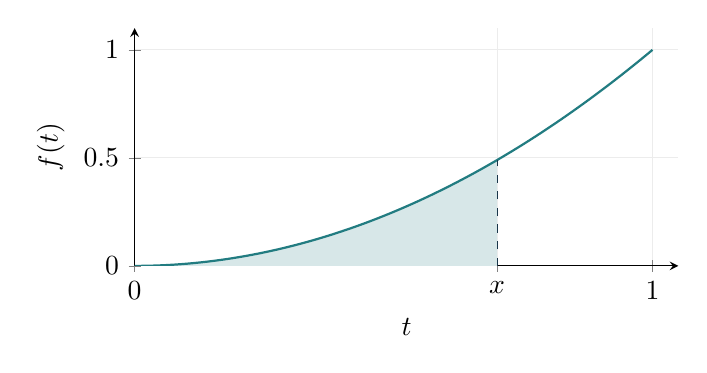
\begin{tikzpicture}
\begin{axis}[width=.7\linewidth,height=4.6cm,
  axis lines=left,xlabel={$t$},ylabel={$f(t)$},
  xmin=0,xmax=1.05,ymin=0,ymax=1.1,
  xtick={0,.7,1},xticklabels={$0$,$x$,$1$},
  grid=major,grid style={gray!15}]
  \addplot[draw=none,fill=Teal!18,domain=0:.7,samples=81]{x^2}\closedcycle;
  \addplot[Teal,thick,domain=0:1,samples=101]{x^2};
  \addplot[Ink,dashed] coordinates {(.7,0)(.7,.49)};
\end{axis}
\end{tikzpicture}
\caption{平方函数下面的面积随右端点移动}\label{fig:area}
\end{figure}

对内部点 \(x\)，令 \(h\to0\) 且 \(x+h\in[a,b]\)。
\begin{align}
  \frac{A(x+h)-A(x)}{h}
    &=\frac{1}{h}\int_x^{x+h}f(t)\,\dd t \notag\\
    &=f(x)+\frac{1}{h}\int_x^{x+h}[f(t)-f(x)]\,\dd t.
\end{align}
把 \(x\) 与 \(x+h\) 之间的闭区间记为 \(I_h\)，误差满足
\[
  \left|\frac{1}{h}\int_x^{x+h}[f(t)-f(x)]\,\dd t\right|
  \leq\max_{t\in I_h}|f(t)-f(x)|\longrightarrow0.
\]
所以 \(A'=f\)。由 \((F-A)'=0\) 得到两者之差为常数，
再代入端点，就得到式~\eqref{eq:ftc}。

\begin{methodbox}{变端点积分求导}
设 \(u,v\) 可导，且取值落在 \(f\) 的同一连续区间内，则
\[
  \frac{\dd}{\dd x}\int_{u(x)}^{v(x)}f(t)\,\dd t
  =f(v(x))v'(x)-f(u(x))u'(x).
\]
\end{methodbox}
\begin{align*}
  \int_0^1x^2\,\dd x&=\left.\frac{x^3}{3}\right|_0^1=\frac13,\\
  \frac{\dd}{\dd x}\int_0^{x^2}\mathrm{e}^t\,\dd t&=2x\mathrm{e}^{x^2},\\
  \frac{\dd}{\dd x}\int_x^{2x}t^2\,\dd t&=7x^2.
\end{align*}
\begin{pitfallbox}
上限是 \(x^2\) 时，别漏乘 \(2x\)。积分跨过奇点时，
先判断积分是否存在，不能直接跨零点对 \(1/x\) 套端点代入。
\end{pitfallbox}

\section{线性代数：从方程组到最小二乘}\label{ch:linear}
\begin{conceptbox}{先把维数写清楚}
\[
  \begin{cases}x+y=3,\\2x-y=0\end{cases}
  \quad\Longleftrightarrow\quad
  \begin{pmatrix}1&1\\2&-1\end{pmatrix}
  \begin{pmatrix}x\\y\end{pmatrix}
  =\begin{pmatrix}3\\0\end{pmatrix}.
\]
消元得 \(3x=3\)，因此 \((x,y)=(1,2)\)。把结果代回两个方程检查。
\end{conceptbox}

\subsection{三个点拟合一条直线}
取演示点 \((0,1),(1,2),(2,2)\)，拟合 \(y\approx a+bt\)。
\[
  A=\begin{pmatrix}1&0\\1&1\\1&2\end{pmatrix},\quad
  \bm{\beta}=\begin{pmatrix}a\\b\end{pmatrix},\quad
  \bm{y}=\begin{pmatrix}1\\2\\2\end{pmatrix}.
\]
这里 \(A\) 为 \(3\times2\)，未知向量为 \(2\times1\)。
\begin{align}
  J(\bm{\beta})
    &=(\bm{y}-A\bm{\beta})^{\mathsf T}(\bm{y}-A\bm{\beta}),\notag\\
  \nabla J(\bm{\beta})
    &=2A^{\mathsf T}A\bm{\beta}-2A^{\mathsf T}\bm{y}.\label{eq:gradient}
\end{align}
令梯度为零，得到正规方程
\[
  \begin{pmatrix}3&3\\3&5\end{pmatrix}\widehat{\bm{\beta}}
  =\begin{pmatrix}5\\6\end{pmatrix},\qquad
  \widehat{\bm{\beta}}=\begin{pmatrix}7/6\\1/2\end{pmatrix}.
\]
因 \(A\) 列满秩，\(A^{\mathsf T}A\) 正定，解是唯一的最小值点。

\begin{table}[htbp]
\centering
\caption{拟合结果与残差：数据仅用于演示}\label{tab:fit}
\begin{tabular}{cccc}
\toprule
\(t\) & 观测值 & 拟合值 & 残差（观测减拟合） \\
\midrule
0 & 1 & \(7/6\) & \(-1/6\) \\
1 & 2 & \(5/3\) & \(1/3\) \\
2 & 2 & \(13/6\) & \(-1/6\) \\
\bottomrule
\end{tabular}
\end{table}
\[
  \mathrm{SSE}=\left(-\frac16\right)^2+
    \left(\frac13\right)^2+\left(-\frac16\right)^2=\frac16.
\]
\begin{methodbox}{最小二乘的检查顺序}
列出设计矩阵，核对维数，检查列秩，再求解正规方程。
算完用 \(A^{\mathsf T}(\bm{y}-A\widehat{\bm{\beta}})=\bm0\) 检查。
数值计算中可用 QR 或 SVD，避免把显式求逆当成唯一算法。
\end{methodbox}
\begin{pitfallbox}
\(A\) 不是方阵，不能直接求 \(A^{-1}\)。
正规方程有唯一解需要列满秩；矩阵乘法也不能任意交换顺序。
\end{pitfallbox}

\section{概率论：把积分与拟合接起来}\label{ch:probability}
\subsection{用积分求均值与方差}
\begin{conceptbox}{均匀分布的一次完整计算}
若 \(X\sim U(0,1)\)，则分布函数为
\[
  F_X(t)=\begin{cases}
    0,&t<0,\\
    t,&0\leq t<1,\\
    1,&t\geq1.
  \end{cases}
\]
区间内的密度为 1。
\end{conceptbox}
\begin{align*}
  \E[X]&=\int_0^1x\,\dd x=\frac12,\\
  \E[X^2]&=\int_0^1x^2\,\dd x=\frac13,\\
  \operatorname{Var}(X)&=\E[X^2]-(\E[X])^2=\frac1{12}.
\end{align*}
第二行正好复用了高数部分的定积分，但现在还要乘相应的概率密度。

\subsection{给最小二乘补上随机误差假设}
把线代部分扩展为模型 \(\bm{y}=A\bm{\beta}+\bm{\varepsilon}\)，
其中 \(A\) 固定且列满秩，并假设
\[
  \E[\bm{\varepsilon}]=\bm0,\qquad
  \Cov(\bm{\varepsilon})=\sigma^2 I.
\]
把 \(\widehat{\bm{\beta}}=(A^{\mathsf T}A)^{-1}A^{\mathsf T}\bm{y}\) 代回模型，得到
\begin{align*}
  \widehat{\bm{\beta}}
    &=\bm{\beta}+(A^{\mathsf T}A)^{-1}A^{\mathsf T}\bm{\varepsilon},\\
  \E[\widehat{\bm{\beta}}]&=\bm{\beta},\\
  \Cov(\widehat{\bm{\beta}})&=\sigma^2(A^{\mathsf T}A)^{-1}
    =\frac{\sigma^2}{6}\begin{pmatrix}5&-3\\-3&3\end{pmatrix}.
\end{align*}
这些均值与协方差结论不要求误差服从正态分布。
在这套误差假设下，演示数据给出残差方差估计
\[
  \widehat{\sigma}^2=\frac{\mathrm{SSE}}{n-p}
  =\frac{1/6}{3-2}=\frac16.
\]
这里仅演示公式，不凭三个点宣称预测可靠。

\begin{methodbox}{三科联动的落点}
高数提供求导与积分；线代组织多个参数；概率说明估计量的不确定性。
每一步都要带上自己的适用条件，而不是只借用公式的外形。
\end{methodbox}
\begin{pitfallbox}
\(\E[X^2]\) 一般不等于 \((\E[X])^2\)。
误差方差估计中的分母是 \(n-p\)，不要未经判断就写成 \(n\)。
\end{pitfallbox}
\end{document}
